% =====================================================================
%  SECTIONS 2-4 — Certificates, architectural admissibility, exact
%  integration. Draft 1.
% =====================================================================

\section{Primal--dual certificates}
\label{sec:primaldual}

Let $Y = [0,1)^2$ be the unit cell, $k \in L^\infty(Y)$ a positive
piecewise-constant coefficient, and $\langle \cdot \rangle$ the average over
$Y$. For a prescribed mean gradient $\bar g$ the corrector $\theta$ solves
$\operatorname{div}\!\big(k(\bar g + \nabla\theta)\big) = 0$ with $\theta$
$Y$-periodic, and the effective tensor admits the variational
characterisation~\cite{Milton2002}
%
\begin{equation}
  \bar g \cdot K_{\mathrm{eff}}\, \bar g
  \;=\; \min_{\theta \in H^1_{\mathrm{per}}(Y)}
  \big\langle (\bar g + \nabla\theta) \cdot k (\bar g + \nabla\theta) \big\rangle .
  \label{eq:primal}
\end{equation}

\subsection{Upper bound}

\begin{theorem}[Primal certificate]
\label{thm:primal}
Let $\chi_1,\chi_2 \in H^1_{\mathrm{per}}(Y)$ be arbitrary and set
$G_i = e_i + \nabla \chi_i$. Then
%
\begin{equation}
  \big[K_{\mathrm{up}}\big]_{ij} := \big\langle k\, G_i \cdot G_j \big\rangle
  \qquad \text{satisfies} \qquad
  K_{\mathrm{up}} \;\succeq\; K_{\mathrm{eff}}
  \label{eq:Kup}
\end{equation}
%
in the L\"owner order.
\end{theorem}

\begin{proof}
Take the load-linear trial family
$\theta(\bar g) = \bar g_1 \chi_1 + \bar g_2 \chi_2$, which is admissible
in~\eqref{eq:primal} for every $\bar g$. Substituting gives
$\bar g \cdot K_{\mathrm{eff}} \bar g \le \bar g^{\!\top} K_{\mathrm{up}} \bar g$
for all $\bar g$, which is the assertion.
\end{proof}
Linearity of the trial map in $\bar g$ is the only structural requirement,
which is why the construction uses one field per unit load and combines
loads by superposition rather than supplying $\bar g$ as a network input.

\subsection{Lower bound}

The complementary principle characterises the inverse,
%
\begin{equation}
  \bar q \cdot K_{\mathrm{eff}}^{-1} \bar q
  \;=\; \min_{\substack{\operatorname{div} q = 0 \\ \langle q \rangle = \bar q}}
  \big\langle q \cdot k^{-1} q \big\rangle .
  \label{eq:dual}
\end{equation}
%
\begin{theorem}[Dual certificate]
\label{thm:dual}
Let $Q_i$ be admissible in~\eqref{eq:dual} with $\langle Q_i \rangle = e_i$.
Then $S_{\mathrm{up}} := \big[\langle k^{-1} Q_i \cdot Q_j\rangle\big]
\succeq K_{\mathrm{eff}}^{-1}$ and consequently
%
\begin{equation}
  K_{\mathrm{low}} := S_{\mathrm{up}}^{-1} \;\preceq\; K_{\mathrm{eff}}
  \;\preceq\; K_{\mathrm{up}} .
  \label{eq:sandwich}
\end{equation}
\end{theorem}

\begin{proof}
The superposition argument of Theorem~\ref{thm:primal} applied
to~\eqref{eq:dual} gives $S_{\mathrm{up}} \succeq K_{\mathrm{eff}}^{-1}$;
inversion reverses the L\"owner order on symmetric positive definite
matrices, and the upper bound is Theorem~\ref{thm:primal}.
\end{proof}

The width of~\eqref{eq:sandwich} is a computable per-instance error
certificate. The construction is classical: it is the hypercircle
argument of Prager and Synge~\cite{PragerSynge1947}, developed for
homogenization by Dvo\v{r}\'ak and Haslinger and realised with exact
integration in a Fourier--Galerkin setting by Vond\v{r}ejc and
co-workers~\cite{Vondrejc2015,Vondrejc2016}, and with guaranteed two-sided
stiffness bounds by Gaynutdinova et al.~\cite{Gaynutdinova2023}. Its neural realisation for
scalar conductivity, including certification by projection onto conforming
finite elements, is due to Gaynutdinova et al.~\cite{Gaynutdinova2026}.
Our contribution begins after this point.

We distinguish this construction from the broader literature on computable
error bounds for physics-informed networks, which certifies a \emph{field}
rather than a homogenized tensor: certified wavelet-based
approximations with computable upper bounds~\cite{Ernst2024}. Such results bound the
distance between a network and the solution of a PDE. The certificates here
bound a \emph{functional} of that solution, the effective tensor, from two sides, and do so without any stability or coercivity constant entering
the estimate, because the bounds follow from minimisation rather than from
residual propagation.

\subsection{Elasticity}

In Mandel notation, where strains and stresses are represented as
$(\varepsilon_{11}, \varepsilon_{22}, \sqrt{2}\,\varepsilon_{12})$ and
$(\sigma_{11}, \sigma_{22}, \sqrt{2}\,\sigma_{12})$, the L\"owner order on
stiffness matrices is literal matrix ordering and the compliance is a plain
matrix inverse. With three unit Mandel strains $E_k$ and total strains
$F_k = E_k + \varepsilon(\chi_k)$, and three unit Mandel stresses $T_k$
with statically admissible total stresses $\Sigma_k$,
%
\begin{equation}
  \big[C_{\mathrm{up}}\big]_{kl} = \langle F_k \cdot \mathbb{C} F_l \rangle
  \succeq C_{\mathrm{eff}}, \qquad
  \big[S_{\mathrm{up}}\big]_{kl} = \langle \Sigma_k \cdot \mathbb{S} \Sigma_l \rangle,
  \quad C_{\mathrm{low}} = S_{\mathrm{up}}^{-1} \preceq C_{\mathrm{eff}} .
  \label{eq:elastic}
\end{equation}

\section{Admissibility by architecture}
\label{sec:admissible}

The bounds~\eqref{eq:sandwich} and~\eqref{eq:elastic} hold for
\emph{any} admissible fields. We therefore enforce admissibility
structurally, so that optimisation quality affects tightness rather than
validity. A poorly trained model need not be reliably identified by a wide
interval, but its projected and exactly integrated output remains a valid
certificate whenever the following contract is met.

\paragraph{Periodicity.} Networks receive only the Fourier features
$\{\sin 2\pi m y_c, \cos 2\pi m y_c\}_{m \le M,\, c=1,2}$. Any smooth
function of these is $Y$-periodic, and the mean of the gradient of a
periodic field vanishes identically.

\paragraph{Primal fields.} One scalar head per unit load (two for
conductivity, six for plane-strain elasticity: three loads times two
displacement components) supplies $\chi_i$ directly; the trial family is
linear in the load by construction, as~\eqref{eq:Kup} requires.

\paragraph{Scalar dual.} Writing the flux fluctuation as the rotated
gradient of a periodic stream function,
$q = \bar q + \operatorname{curl}\psi$ with
$\operatorname{curl}\psi = (\partial_2 \psi, -\partial_1 \psi)$, gives
$\operatorname{div} q = \psi_{,21} - \psi_{,12} = 0$ identically and
$\langle \operatorname{curl}\psi\rangle = 0$ exactly. Both constraints
of~\eqref{eq:dual} are thus satisfied by construction rather than by
penalty. This is the construction of~\cite{Gaynutdinova2026}.

\paragraph{Tensor dual.} In two dimensions the Airy representation
%
\begin{equation}
  \sigma'_{11} = \varphi_{,22}, \qquad
  \sigma'_{22} = \varphi_{,11}, \qquad
  \sigma'_{12} = -\varphi_{,12}
  \label{eq:airy}
\end{equation}
%
is symmetric, divergence-free identically, and has exactly zero mean for
periodic $\varphi$, since the mean of any second derivative of a periodic
field vanishes. Three potentials, one per unit Mandel stress, therefore
give statically admissible $\Sigma_k$ with exactly the prescribed means.
The corresponding classical construction, a self-equilibrated stress field
generated from a stress potential and discretised with $C^1$
Bogner--Fox--Schmit elements, is due to Gaynutdinova et
al.~\cite{Gaynutdinova2023}; we carry it onto neural trial fields.

\paragraph{Initialisation.} Zero-initialising the output layers makes the
trial fluctuations vanish, so the certificate at step zero is exactly the
Voigt--Reuss envelope (Figure~\ref{fig:convergence}): $K_{\mathrm{up}} = \langle k \rangle I$ and
$K_{\mathrm{low}} = \langle k^{-1}\rangle^{-1} I$. Validity therefore holds
from the first iteration and training can only tighten.

\begin{figure}[t]
\centering
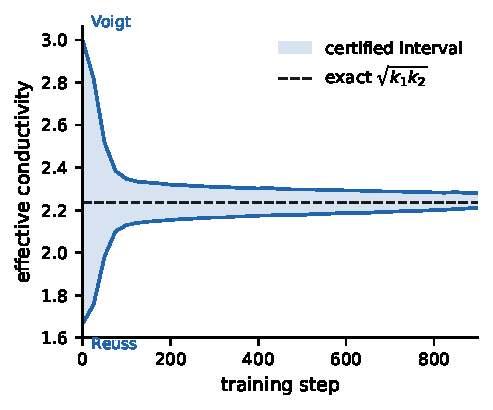
\includegraphics[width=0.62\linewidth]{figures/fig_convergence.pdf}
\caption{Certified bounds closing from the Voigt--Reuss envelope onto the
exact effective conductivity of a two-phase checkerboard. Zero-initialised
output layers make the first iterate exactly the classical envelope, and
every subsequent iterate is a valid certificate; training tightens the
interval but is not required for validity.}
\label{fig:convergence}
\end{figure}

\paragraph{Objective.} Since each head appears in exactly one term of
$\operatorname{tr} K_{\mathrm{up}} + \operatorname{tr} S_{\mathrm{up}}$ and
is minimised by the corresponding true corrector, minimising this sum
tightens both bounds simultaneously. No reference solutions enter training;
finite-element and FFT solvers are used only to audit the implementation.

\section{Exact-integration certification}
\label{sec:exact}

The bounds are statements about integrals, and a scheme that evaluates them
by sampling inherits the quadrature error, which Section~\ref{sec:quadrature} shows can be severe enough to invalidate a
certificate. We remove the dependence entirely by interpolating the trained
fields into conforming finite-element spaces on a mesh aligned with the
phase boundaries and integrating exactly. The network proposes; the
projection certifies.

\paragraph{Primal.} Nodal $Q_1$ interpolation of a continuous periodic
field is continuous, piecewise bilinear and periodic, hence lies in a
conforming subspace of $H^1_{\mathrm{per}}$, and~\eqref{eq:Kup} applies
verbatim.

\paragraph{Scalar dual.} Let $\psi_h$ be continuous piecewise bilinear and
$q = \operatorname{curl}\psi_h$. Within each element
$\operatorname{div} q = 0$ pointwise. Across an element edge, continuity of
$\psi_h$ forces its \emph{tangential} derivative to be continuous, and the
curl rotates tangential into normal, so the \emph{normal} component of $q$
is continuous, which is precisely the condition for $q \in H(\operatorname{div})$
with vanishing divergence. Interpolation therefore certifies the dual side
with no need for $H(\operatorname{div})$-conforming elements.

\paragraph{Tensor dual.} The $Q_1$ space cannot carry an Airy stress, since
bilinear functions have $\varphi_{,11} = \varphi_{,22} = 0$ identically. We
use the Bogner--Fox--Schmit bicubic Hermite space, with nodal degrees of
freedom $(\varphi, \varphi_{,x}, \varphi_{,y}, \varphi_{,xy})$, all four
obtained exactly by automatic differentiation of the network. Global $C^1$
continuity is what makes the interpolated stress admissible: across an edge
with normal $e_1$ the traction components are
$(\varphi_{,22}, -\varphi_{,12})$; $\varphi_{,22}$ is a second tangential
derivative of a continuous function, and $\varphi_{,12}$ is the tangential
derivative of $\varphi_{,1}$, which is continuous by $C^1$ regularity.
Traction is therefore continuous, the interpolated stress lies in
$H(\operatorname{div})$ with vanishing divergence, and its cell mean is
exact.

\paragraph{Exactness of the quadrature.} On a phase-aligned mesh the
coefficient is constant per element. Gradients of $Q_1$ fields are
bilinear, so the primal integrand has degree at most two per coordinate and
$2\times 2$ Gauss is exact. Second derivatives of BFS fields have degree at
most three per coordinate, so the complementary integrand has degree at
most six and $4 \times 4$ Gauss, exact to degree seven, suffices. The
resulting certificates hold up to floating-point arithmetic only.

\begin{proposition}[Certification contract]
\label{prop:contract}
For each reported input, the bounds in \eqref{eq:sandwich} and
\eqref{eq:elastic} are certified for the discretised periodic problem if:
(i) every phase coefficient is uniformly positive definite; (ii) the
certification mesh resolves every phase boundary, so the coefficient is
constant on each element; (iii) the projected primal fields are periodic
and belong to the stated conforming $H^1$ spaces; (iv) the projected dual
fields have the prescribed cell means and belong to $H(\operatorname{div})$
with zero divergence; and (v) the stated elementwise Gauss rules are used.
The conclusion is subject only to floating-point round-off.
\end{proposition}

\begin{proof}
Conditions (iii) and (iv) make the primal and complementary trial fields
admissible in the variational principles. Theorems~\ref{thm:primal} and
\ref{thm:dual}, and their elasticity analogues, then give the L\"owner
ordering. Conditions (i), (ii), and (v) ensure that the assembled energy
integrals are the exact finite-element integrals described above.
\end{proof}

\paragraph{Verification.} Table~\ref{tab:anchors} reports the
machine-precision anchors, obtained by feeding closed-form optimal fields
through the production assembly. Because the analytic correctors are
elementwise polynomial, interpolation is exact and any discrepancy would
indicate an implementation error rather than an approximation.

\begin{table}[t]
\centering
\caption{Machine-precision verification. Closed-form optimal fields passed
through the production code path must reproduce the exact effective tensor.}
\label{tab:anchors}
\resizebox{\textwidth}{!}{%
\begin{tabular}{llll}
\toprule
projection & space & anchor & agreement \\
\midrule
scalar primal and dual & $Q_1$ ($C^0$) & rank-one laminate & $10^{-12}$ \\
elasticity primal & $Q_1$ vector & elastic laminate & $10^{-11}$ \\
elasticity dual & BFS bicubic Hermite ($C^1$) & Airy potential of the laminate & $10^{-10}$ \\
\bottomrule
\end{tabular}}
\end{table}

One normalisation deserves record, since it caused an error during
development that the anchors detected. The stress fields associated with
the \emph{strain}-basis solutions have mean stress $C_{\mathrm{eff}}$
rather than the unit basis, so their compliance-weighted Gram matrix is
$C_{\mathrm{eff}}$ itself and inverting it returns
$C_{\mathrm{eff}}^{-1}$. Analytic or imported trial stresses must therefore
be recombined to unit mean, $\Sigma(T_j) = \sum_k [C_{\mathrm{eff}}^{-1}]_{kj}
\sigma^{(k)}$, before entering~\eqref{eq:elastic}. The network path is
immune, its trial means being the unit $T_k$ by construction.
